\documentclass[article]{jss}

%%%%Re-organization based on SRB notes
%%%%
%%Intro
%%Ecosystem Networks purpose and structure of models
%%1.network ecology
%%2.ENA
%%3.previous software and enaR
%%ENA network models
%%1. describe models
%%2. model construction
%%3. mathematical description
%%ENA analyses
%%1. provided models
%%2. visualization
%%3. model input
%%4+. analyses
%%n. batch processing
%%Conclusion
%%1.Connecting to other packages
%%2.Future directions
%%3.Contributing

%%%%%%%%%%%%%%%%%%%%%%%%%%%%%%
%% declarations for jss.cls %%%%%%%%%%%%%%%%%%%%%%%%%%%%%%%%%%%%%%%%%%
%%%%%%%%%%%%%%%%%%%%%%%%%%%%%%

%% almost as usual
\author{Matthew K. Lau\\ Harvard Forest\\Harvard University \And
        Stuart R. Borrett\\Department of Biology and Marine Biology\\
        University of North Carolina Wilmington\\and\\Duke Network
        Analysis Center, Social Science Research Institute \\ Duke University}
\title{enaR: Ecosystem Network Analysis with R}

%% for pretty printing and a nice hypersummary also set:
\Plainauthor{Matthew K. Lau, Stuart R. Borrett} %% comma-separated
\Plaintitle{enaR: Ecosystem Network Analyses with R} %% without formatting
\Shorttitle{\pkg{enaR}: Ecosystem Network Analyses with R} %% a short title (if necessary)

%% an abstract and keywords
\Abstract{
  Ecosystem Network Analysis (ENA) provides a framework for
  investigating the structure, function and dynamics of ecological
  systems, primarily ecosystem models with physically conserved
  units. We present the \textit{enaR} package, which provides a
  broad representation of many of the core tools developed by the ENA
  community, detailing how to use the primary functions of the package
  for the analysis of single models or simultaneous, synthetic
  analysis of multiple ecosystem models.
}
\Keywords{ecology, ENA, ecosystems, species interactions, networks, \proglang{R}}
\Plainkeywords{ecology, ENA, ecosystems, species interactions, networks, R} %% without formatting
%% at least one keyword must be supplied

%% publication information
%% NOTE: Typically, this can be left commented and will be filled out by the technical editor
%% \Volume{50}
%% \Issue{9}
%% \Month{June}
%% \Year{2012}
%% \Submitdate{2012-06-04}
%% \Acceptdate{2012-06-04}

%% The address of (at least) one author should be given
%% in the following format:

\Address{
  Matthew K. Lau\\
  Harvard Forest\\
  Harvard University\\
  324 N Main St, Petersham, MA 01366, USA\\
  E-mail: \email{matthewklau@fas.harvard.edu}\\
  URL: \url{https://github.com/MKLau}\\
  \\
  Stuart R. Borrett\\
  Department of Biology and Marine Biology\\
  University of North Carolina Wilmington\\
  601 South College Road, Wilmington, NC 28403, USA\\
  E-mail: \email{borretts@uncw.edu}\\
  URL: \url{http://people.uncw.edu/borretts/}
}

%% It is also possible to add a telephone and fax number
%% before the e-mail in the following format:
%% Telephone: +43/512/507-7103
%% Fax: +43/512/507-2851

%% for those who use Sweave please include the following line (with % symbols):
%% need no \usepackage{Sweave.sty}

\usepackage[super, sort]{natbib}
  \bibpunct{(}{)}{;}{a}{,}{,} % required for natbib
\usepackage{ucs} %needed for R output: signif stars etc, quotes
\usepackage[utf8x]{inputenc}
\usepackage[T1]{fontenc}
\usepackage{sidecap}

%% end of declarations %%%%%%%%%%%%%%%%%%%%%%%%%%%%%%%%%%%%%%%%%%%%%%%


\begin{document}

%% include your article here, just as usual
%% Note that you should use the \pkg{}, \proglang{} and \code{} commands.

%%%Ecological Networks introductory paragraph

\section[Ecosystem Network Analysis]{Ecosystem Network Analysis}
%% Note: If there is markup in \(sub)section, then it has to be escape as above.

Ecosystem Network Analysis (ENA) is a family of algorithms for
investigating the structure and function of ecological systems
\cite{borrett12_netecol,ulanowicz86,fath99_review}.  These systems are
modeled as thermodynamically conserved energy--matter exchanges
between species, groups of species, or non-living componets (e.g.,
dead organic matter) of the ecosystem, and the weighted, directed
edges are the quantified transfers of energy or matter.

% need a paragraph that introduces the 2 worlds of ena

% objectives
Disparate software packages have been created to support
ENA. Initially algorithms were developed and distributed as the DOS
based NETWRK4 \cite{ulanowicz91}, which is still available from
\url{http://www.cbl.umces.edu/~ulan/ntwk/network.html}.  Some of these
algorithms were reimplemented in an Microsoft Excel based toolbox,
WAND \cite{allesina04_wand}. The popular Ecopath with Ecosim software
that assists with model construction \citep{christensen04} also
provides multiple ENA algorithms.  \citet{fath06}
published NEA.m that collects many ENA algorithms together in a single
MATLAB\copyright function. Although these packages collectively
provide access to a large set of powerful analytical tools, the
fragmented distribution of these algorithms has inhibited the
development of theory and the further implementation of important
algorithms.

The \textit{enaR} package brings together ENA algorithms into one
common software framework that is readily available and extensible.
The package is written in the \R\ language, which is free and
open-source.  Due largely to this, \R\ is now one of the most widely
used analytical programming lanuages in the biological
sciences. \textit{enaR} builds on previously developed tools for
network analysis. For example, it uses the \textit{network} data
structure developed by \citet{butts08_network} and the network
analysis tools built into the \textit{network}, \textit{sna} (social
network analysis) \citep{butts08_social}, and other packages
collectively called \textit{statnet} \citep{handcock2008statnet}. In
this article we introduce the user to ENA concepts and algorithms,
provide description of how to input ecosystem network models and give
detailed description of how to conduct these analyses using
\textit{enaR}.







%% <<z,echo=false>>=
%% # set plotting parameters
%% opar <- par(las=1,mar=c(0,0,0,0),xpd=TRUE,bg="white")

%% ## Taken from https://stat.ethz.ch/pipermail/r-devel/2011-September/062126.html
%% if (all(ls()!='f.list')){
%%   require(codetools)
%% library(enaR)
%% called.by <- function(tarFunc, tarPack){
%%   flist <-   sapply(lsf.str(tarPack, all=TRUE), c)
%%   names(flist) <- NULL
%%   gotit <- sapply(flist, function(x) tarFunc %in% findGlobals(get(x, tarPack),FALSE)$functions)
%%   flist[gotit]
%% }

%% f.list <- as.character(sapply(lsf.str('package:enaR',all=TRUE),c))
%% f.array <- array(0,dim=rep(length(f.list),2))
%% rownames(f.array) <- colnames(f.array) <- f.list
%% for (i in 1:length(f.list)){
%%   f.array[match(called.by(f.list[i],'package:enaR'),rownames(f.array)),i] <- 1
%% }
%% f.net <- network(t(f.array))
%% }

%% plot(f.net,displaylabels=TRUE,label.cex=0.85,arrowhead.cex=0.65,
%%      edge.lwd=0.75,vertex.col='lightblue',vertex.border='white',edge.col='darkgrey')
%% @



\begin{figure}
  \center
%% <<fig=true,echo=false>>=
%% <<z>>
%% @
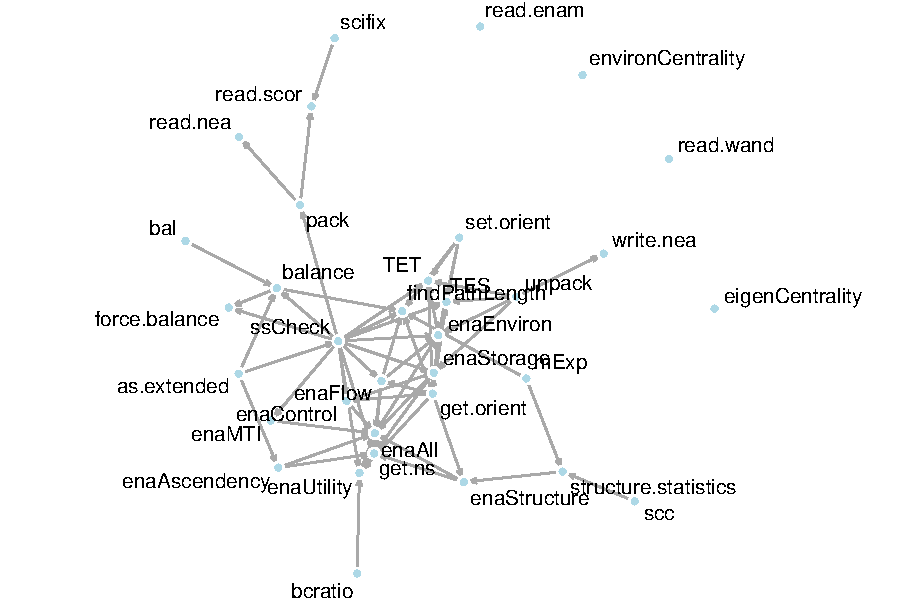
\includegraphics[]{enaR-vignette-003}
\caption{A plot of the \textit{enaR} function relationships. Edges
  point \textit{from} a function that provides information \textit{to}
  the function that receives that information.} \label{fig:fig}
\end{figure}

% % use
% The analysis has been used in a variety of ways, including to show
% the relative importance of indirect effects in ecosystems
% \citep{patten83, higashi89, salas11_did} and their capacity to
% effectively transform the relations among organisms
% \citep{ulanowicz90, patten91, fath98, bondavalli99}.  From these
% applications a new theoretical understanding of ecosystems has
% emerged \citep{higashi91, belgrano05, jorgensen07_newecology}.
% Recently, scientists have been applying these methods to understand
% trophic dynamics in the Sylt-R{\o}m{\o} Bight
% \citep{baird04_sylt,baird08_sylt}, biogeochemical cycling in
% estuaries \cite{christian03, hines12}, and urban sustainability
% \citep{zhang10, chen12}.

\section{Data Input: General}
In this section we describe the data necessary for the Ecological
Network Analysis and show how to build the central network data object
in \R\ that contains the model data for subsequent analysis.  To
start, we assume you have installed the enaR package, and then loaded
the library as follows:

%%%%% Getting Set Up %%%%%%%%%%%
\setkeys{Gin}{width=0.55\linewidth}


% Show loading the library and listing the functions in the package
\begin{Schunk}
\begin{Sinput}
> library(enaR)
\end{Sinput}
\end{Schunk}
%%%%%%%%%%%%%%%%%%%%%%%%%%%%%%%%%

\subsection{Model Data} \label{sec:data}
ENA is applied to a network model of energy--matter exchanges among
system components.  The system is modeled as a set of $n$ compartments
or nodes that represent species, species-complexes (i.e., trophic
guilds or functional groups), or non-living components of the system
in which energy--matter is stored.  Nodes are connected by $L$
observed fluxes, termed directed edges or links.  This analysis
requires an estimate of the energy--matter flowing from node $i$ to
$j$ over a given period, $\mathbf{F}_{n\times n}=[f_{ij}]$,
$i,j=1,2,\ldots,n$.  These fluxes can be generated by any process such
as feeding (like a food web), excretion, and death.  As ecosystems are
thermodynamically open, there must also be energy--matter inputs into
the system $\mathbf{z}_{1 \times n}=[z_i]$, and output losses from the
system $\mathbf{y}_{1 \times n}=[y_i]$.  While the Patten School treats
all outputs the same, the Ulanowicz School typically partitions
outputs into respiration $\mathbf{r}_{1\times n}=[r_i]$ and export
$\mathbf{e}_{1\times n}=[e_i]$ to account for differences in energetic
quality. Note that $y_i = r_i + e_i, \forall i$.  Some analyses
also require the amount of energy--matter stored in each node (e.g.,
biomass), $\mathbf{X}_{1\times n}=[x_i]$.  The final required
information is a categorization of each node as living or not, which
is essential for algorithms from the Ulanowicz School.  For
our implementation, we have created a logical vector $\mathbf{Living}_{1 \times
  n}$ that indicates whether the $i^{th}$ node is living (TRUE)
or not (FALSE).  Together, the model data $\mathcal{M}$ can be
summarized as $\mathcal{M} =
\{\mathbf{F}, \mathbf{z}, \mathbf{e}, \mathbf{r}, \mathbf{X}, \mathbf{Living}\}$.


% Orientation
The ENA methodology is an application and extension of economic
Input--Output Analysis \citep{leontief1936,leontief66} that was first
introduced into ecology by \citet{hannon73}.  Two major schools have
developed in ENA.  The first is based on Dr.\ Robert E.\ Ulanowicz's
work with a strong focus on trophic dynamics and a use of information
theory \citep{ulanowicz86, ulanowicz97, ulanowicz04}.  The second
school has an environment focus and is built on the environ concept
introduced by Dr.\ Bernard C.\ Patten \citep{patten76, patten78,
  fath99_review}.  Patten's approach has been collectively referred to
separately as \emph{Network Environ Analysis}. At the core the two
approaches are very similar; however, they make some different
starting assumptions and follow independent yet braided development
tracks. One example difference that has historically inhibited
collaboration and applications is that the two schools orient their
analytical matrices in different ways.  The Ulanowicz school orients
their matrices as flows from rows-to-columns, which is the most common
orientation in the broader field of network science
\citep[e.g.,][]{brandes05}.  In contrast, the Patten School has
historically oriented their matricies from column-to-row.  Recent
research has started to bring the work of the two schools back
together \citep[e.g.,][]{scharler09comparing}; we hope this software
contributes to this.

Notice the row-to-column orientation of $\mathbf{F}$.  This is
consistent with the Ulanowicz School of network analysis, as well as
the orientation commonly used in Social Network Analysis and used in
the \textit{statnet} packages.  However, this is the opposite
orientation typically used in the Patten School of analysis that
conceptually builds from a system of differential equations and thus
uses the column-to-row orientation common in this area of
mathematics. Even though the difference is only a matrix transpose,
this single difference may be the source of much confusion in the
literature and frustration on the part of users.  We have selected to
use row-to-column orientation for our primary data structure, as it is
the dominant form across network analytics as evidenced by it use in
the \textit{statnet} packages. The package algorithms also return the
results in the row-to-column orientation by default; however, we have
built in functionality with the functions \texttt{get.orient} and
\texttt{set.orient}  that allows users
to return output in the Patten School row-to-column orientation
(see Section~\ref{sec:orient} for details).

% % Assumptions
% To validly apply flow analysis, the network model must meet two
% analytical assumptions.  First, the model must trace a single,
% thermodynamically conserved currency such as energy, carbon, or
% nitrogen.  Second, the model must be at steady-state for many of the
% analyses.  This means that the sum of the energy--matter flowing into
% a node equals that exiting the node such that its storage or biomass
% is not changing.  \citet{fath07_netconstruction} offer further
% suggestions for better ecosystem network model construction.

% Network Data Object
\subsection{Network Data Class}

The \textit{enaR} package stores the model data in the \textbf{network}
class defined in the \textit{network} package \citep[see][for
details]{butts08_network}. Again, the primary network object
components are:

\begin{itemize}
\item F = flow matrix oriented row-to-column
\item z = inputs
\item r = respiration
\item e = exports
\item y = respiration+exports
\item X = biomass or storage values
\item Living = logical vector indicating if the node is living
  (TRUE) or non-living (FALSE)
\end{itemize}

\subsection{Building a Network Object}
Users can assemble the necessary data elements described in
Section~\ref{sec:data} and then use the \texttt{pack} function to create the
network data object.  Here is an example of doing this with
hypothetical data.

%% PACK A MODEL
\begin{Schunk}
\begin{Sinput}
> # generate the flow matrix
> flow.mat <- array(abs(rnorm(100,4,2))*sample(c(0,1),100,replace=TRUE),
+                   dim=c(4,4))
> # name the nodes
> rownames(flow.mat) <- colnames(flow.mat) <- paste('node',(1:nrow(flow.mat)),sep='')
> # generate the inputs
> inputs <- runif(nrow(flow.mat),0,4)
> # generate the exports
> exports <- inputs
> # pack
> fake.model <- pack(flow=flow.mat,
+                    input=inputs,
+                    export=exports,
+                    living=TRUE)
> # model
> fake.model
\end{Sinput}
\end{Schunk}

Unfortunately, the attributes() function does not clearly identify the
network data objects we are using.

\begin{Schunk}
\begin{Sinput}
> attributes(fake.model)
> 
\end{Sinput}
\end{Schunk}

However, individual components can be extracted from the data object
using the form specified in the \textit{network} package.  For
example, we can pull out node of vertex attributes as follows:

\begin{Schunk}
\begin{Sinput}
> fake.model%v%'output'
> fake.model%v%'input'
> fake.model%v%'living'
\end{Sinput}
\end{Schunk}

The network flows are stored as edge weights in the network object,
which lets users fully manipulate the network object with the
\texttt{network} functions.  The flow matrix can be extracted from the
object as

\begin{Schunk}
\begin{Sinput}
> as.matrix(fake.model,attrname="flow")
\end{Sinput}
\end{Schunk}

There are times that it is useful to extract all of the ecosystem
model data elements from the network data object.  This can be
accomplished using the \texttt{unpack} function. The \texttt{unpack}
output is as follows:

\begin{Schunk}
\begin{Sinput}
> unpack(fake.model)
\end{Sinput}
\end{Schunk}

Note that we did not specify the storage values. In these instances
\texttt{pack} produces \texttt{NA} values. Although the package is
designed to help users navigate missing data issues be sure to check
that you are providing the appropriate input for a given function. For
more information, see the help file for the function in question.

%%%%%%%%%%%%%%%%%%%%%
\subsection{Balancing for Steady-State}

Many of the ENA functions assume that the network model is at
steady-state (node inputs equal node outputs).  Thus, this package has
functions for (1) checking to see if the assumption is met and (2)
automatically balancing the model so that input equal outputs.

To determine if the model is balanced and then balance it if necessary:
\begin{Schunk}
\begin{Sinput}
> ## --- Check to see if the model is balanced ---#
> ssCheck(fake.model)
> ## --- To BALANCE a model if needed --- #
> fake.model <- balance(fake.model,method="AVG2")
> ## --- To FORCE BALANCE a model if needed --- #
> fake.model <- force.balance(fake.model)
\end{Sinput}
\end{Schunk}

The automated balancing routines are based on those presented in
\citet{allesina03}.  These authors compare alternative balancing
algorithms and further discuss the implications of using automated
procedures.  Caution is warranted when using these techniques, as they
indiscriminately alter the model flow rates.

%%%%%%%
\section{Data Input: Reading Common Data File Formats}
Several software packages exist in the literature for running ENA.  For
convenience, we have written functions to read in a few of the more
common data formats used by these software.

\subsection*{SCOR}
The \texttt{read.scor} function reads in data stored in the SCOR
format specified by \citet{ulanowicz91} that is the input to the
NETWRK4 programs.  This function can be run as follows.

\begin{Schunk}
\begin{Sinput}
> scor.model <- readLines('http://people.uncw.edu/borretts/data/oyster.dat')
> m <- read.scor(scor.model,from.file=FALSE)
\end{Sinput}
\end{Schunk}

This constructs the network data object from the SCOR file that stores
the ecosystem model data for an oyster reef model \citep{dame81}.  The
individual model elements are

\begin{Schunk}
\begin{Sinput}
> unpack(m)
\end{Sinput}
\end{Schunk}

This same data is stored as a network data object that is distributed
with this package, which can be accessed as:
\begin{Schunk}
\begin{Sinput}
> data(oyster)
> m <- oyster
\end{Sinput}
\end{Schunk}

\subsection*{WAND}
In part to make ENA more accessible to biologists,
\citet{allesina04_wand} recoded some of Ulanowicz's NETWRK4 algorithms
into a Microsoft Excel based tool called WAND.  For this tool, the
model data is stored as a separate Excel file with two worksheets.
The first contains many of the node attributes and the second contains the
flow matrix.  The \texttt{read.wand} function will create an \R\
network data object from a WAND model file. An example WAND file can
be found at \url{http://people.uncw.edu/borretts/data/MDmar02_WAND.xls}.

\begin{Schunk}
\begin{Sinput}
>   m <- read.wand('./MDmar02_WAND.xls')
\end{Sinput}
\end{Schunk}

This code creates a network data object for \textit{enaR} from the WAND
formatted Mdloti ecosystem model data
\citep{scharler2012ecosystem}. This data is courtesy of U.M. Scharler.

\subsection*{ENAM}

Another commonly used data format stores the necessary model data in a
csv or Excel formatted file.  We include an example Excel file of the
Mdloti estuary stored in this form (``MDMAR02.xlsx'', courtesy
of U. M. Scharler).  This format has not been described technically in
the literature nor has it been named.  We refer to it as ENAM as it is
the ENA model data stored primarily as a square matrix with several
preliminary rows that include meta-data, the number of nodes, and
number of living nodes (similar to SCOR).  The data format is
generally similar in concept, if not exact form, to the data system
matrix used as the input to the NEA.m function \citep{fath06}.
However, the ENAM format includes information on whether nodes are
living and partitions output into respiration and exports.

Using an example data file,
\url{http://people.uncw.edu/borretts/data/MDMAR02.xlsx}, this data
format can be read into the \textit{enaR} package as:

\begin{Schunk}
\begin{Sinput}
>   m <- read.enam('./MDMAR02.xlsx')
\end{Sinput}
\end{Schunk}

The current read.enam function assumes the data are stored on the
first worksheet of an Excel file. In the future, we expect to expand
this function's capabilities to read the data from a CSV file.

\subsection*{NEA}

For their Matlab function to perform network environ analysis (Patten School),
\citet{fath06} packaged the model flows, inputs, outputs, and storage
values into what they called a system matrix
\begin{align}
\mathbf{S} = \left[ \begin{array}{ccc} \mathbf{F} & \vec{z} & \vec{X} \\
     \vec{y}  &  0 & 0 \end{array}
\right]_{(n+1) \times (n+2)}.
\end{align}
Flows in the system matrix are oriented from column to row.

The \textit{enaR} function \texttt{read.nea} reads in data with this
format stored as a comma separated value file.  The function
\texttt{write.nea()} will write any network model to a CSV file with
this format.

While convenient, this data format does not enable inclusion of the
full range of model information included in the \textit{enaR} network
data object.  This format does not partition outputs into exports and
respiration values, nor does it identify the node labels are their
living status. This missing information will prevent the use of some
\textit{enaR} functions.

Here is an example of using these functions:
\begin{Schunk}
\begin{Sinput}
> data(oyster)
> # write oyster reef model to a csv file
> write.nea(oyster, file.name="oyster.csv")
> # read in oyster reef model data from NEA.m formatted CSV file
> m <- read.nea("oyster.csv")
> 
> # Again, this model object does NOT contain all
> # of the information in the "oyster" data object.
\end{Sinput}
\end{Schunk}

\section{Network Visualization}

The \textit{enaR} package uses the \textit{network} package plot tools. Here is
one example of how to plot a network model. The figure scaling may
need to be adjusted depending on computer and devices. Also note that
the graph only shows internal system flows.

Figure~\ref{fig:oyster} (left) is a very simple example of to plot a
graph of the oyster reef model accomplished with default settings.


\begin{Schunk}
\begin{Sinput}
> data(oyster)  # load data
> m <- oyster
> set.seed(2)    # set random seed to control plot
> plot(m)       # plot network data object (uses plot.network)
\end{Sinput}
\end{Schunk}

We can use the excellent graphics capabilities of \R\ to make fancier
plot of the same data (Fig.~\ref{fig:oyster}(right)).


\begin{Schunk}
\begin{Sinput}
> # set colors to use
> my.col=c("red","yellow",
+   rgb(204,204,153,maxColorValue=255),
+   "grey22")
> F=m%n%'flow'                   # extract flow information for later use.
> f=which(F!=0, arr.ind=T)       # get indices of positive flows
> opar <- par(las=1,bg=my.col[4],xpd=TRUE,mai=c(1.02, 0.62, 0.82, 0.42))
> set.seed(2)                    # each time the plot is called, the
>                                # layout orientation changes.  setting
>                                # the seed ensures a consistent
>                                # orientation each time the plot
>                                # function is called.
> plot(m,
+      vertex.cex=log(m%v%'storage'), # scale nodes with storage
+      label= m%v%'vertex.names',     # add node labels
+      boxed.labels=FALSE,
+      label.cex=0.65,
+      vertex.sides=45,   # to make rounded
+      edge.lwd=log10(abs(F[f])),     # scale arrows to flow magnitude
+      edge.col=my.col[3],
+      vertex.col=my.col[1],
+      label.col="white",
+      vertex.border = my.col[3],
+      vertex.lty = 1,
+      xlim=c(-4,1),ylim=c(-2,-2))
> rm(opar)             # remove changes to the plotting parameters
\end{Sinput}
\end{Schunk}


\begin{figure}
  \center
  \begin{tabular}{cc}
%% <<fig=true,echo=false>>=
%% <<a>>
%% @ \\
%% <<fig=true,echo=false>>=
%% <<b>>
%% @ \\
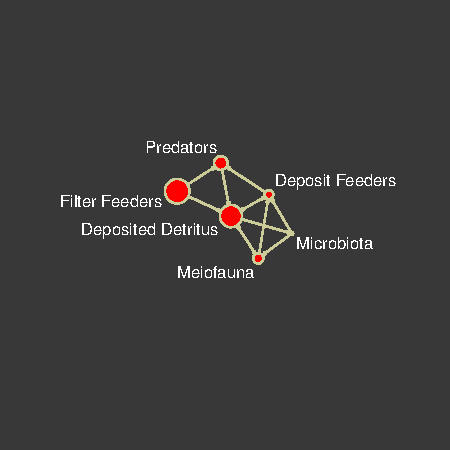
\includegraphics[]{enaR-vignette-020}
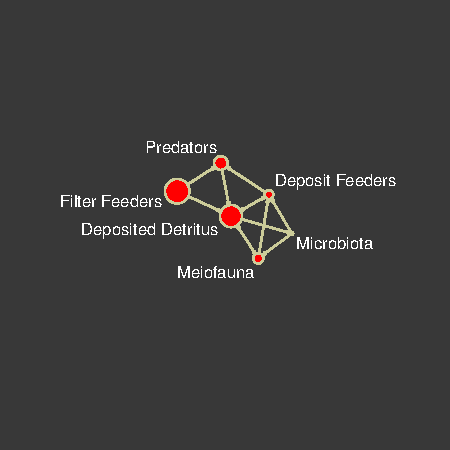
\includegraphics[]{enaR-vignette-021}
  \end{tabular}
  \caption{Simple (left) and fancy (right) plot of the Oyster network
    model (Dame and Patten 1981).} \label{fig:oyster}
\end{figure}



%%%%%%%%

\section{Analyzing Ecosystem Models}

The primary ENA algorithms included in this package are summarized in
Table~\ref{tab:alg} and a plot of the network of functions for the
package can be found in Figure~\ref{fig:fig}.

\begin{table*}
\center
\caption{Primary Ecological Network Analysis algorithms in
  \textit{enaR}.} \label{tab:alg}
\tableline
%\begin{scriptsize}
\begin{tabular}{l l l l l }
\textbf{Analysis} & \textbf{Function Name} & \textbf{School} \\ \hline \\ [-1ex]
Structure & \texttt{enaStructure} & foundational, Patten \\
Flow & \texttt{enaFlow} & foundational, Patten \\
Ascendency & \texttt{enaAscendency} & Ulanowicz \\
Storage & \texttt{enaStorage} & Patten \\
Utility & \texttt{enaUtility} & Patten \\
Mixed Trophic Impacts & \texttt{enaMTI} & Ulanowicz \\
Control & \texttt{enaControl} & Patten \\
Environ & \texttt{enaEnviron} & Patten \\
\end{tabular}
%\end{scriptsize}
\tableline
\end{table*}


In practice, ENA is applied to a single model.  Here, we walk through an
example of applying multiple ENA algorithms to the oyster reef model
\citep{dame81}.  The main ENA algorithms encoded in \textit{enaR} are
summarized in Table~\ref{tab:alg}.

Again, in this package results are reported in the row-to-column
orientation by default -- including the algorithms from the Patten
school.  Please see Section~\ref{sec:orient} for how to change this
default if needed.

\subsection{Structural Network Analysis}
Structural network analysis is common to many types of network
analysis.  The structural analyses applied here are based on those
presented in NEA.m \citep{fath06} following the Patten School.  Output
of the enaStructure function is summarized in Table~\ref{tab:structure}

% STRUCTURE
\begin{table*}[h]
  \caption{Resultant matrices and network statistics returned by the
    \texttt{enaStructure} function in \textit{enaR}.}\label{tab:structure}
\center
\begin{small}
  \begin{tabular}{l l}
    \textbf{Label} & \textbf{Description} \\ \hline \\[-2ex]
    \multicolumn{2}{l}{\textit{Matrices}} \\
    A & $n \times n$ adjacency matrix\\  [1ex]
    \multicolumn{2}{l}{\textit{Network statistics}} \\
    n & number of nodes \\
    L & number of directed edges \\
    C & connectance $(C = L/n^2)$; the proportion of possible directed
    edges connected.\\
    LD & Link Density (L/n) \\
    ppr & estimated rate of pathway proliferation \citep{borrett03} \\
    lam1A & dominant eigenvalue of A ($lambda_1(\mathbf{A})$), which is the \\
    & asymptotic rate of pathway proliferation \citep{borrett07_jtb}\\
    mlam1A & multiplicity of the dominant eigenvalue (number of
    times repeated) \\
    rho & damping ratio, an indicator of how quickly
    $[a_{ij}]^{(m)}/[a_{ij}]^{(m-1)}$ goes to $lam_1(\mathbf{A})$ \citep[][, p. 95]{caswell01} \\
    R & distance of $lam_1(\mathbf{A})$ from the bulk of the eigen spectrum \citep{farkas2001spectra}\\
    d & difference between dominant eigenvalue and link density
    (expected value for random graph) \\
    no.scc & number of strongly connected components (SCC) \\
    no.scc.big & number of SCC with more than one node \\
    pscc & fraction of network nodes included in a big SCC\\
    \hline
  \end{tabular}
\end{small}
\end{table*}

\begin{Schunk}
\begin{Sinput}
> St <- enaStructure(m)
> attributes(St)
> St$ns
\end{Sinput}
\end{Schunk}

The structural network statistics show that the oyster reef model has
6 nodes, a pathway proliferation rate of 2.14, and that the model is
comprised of two strongly connected components but that only one has
more than one node.

\subsection{Flow Analysis}
Flow analysis or throughflow analysis is one of the core ENA analyses
for both the Ulanowicz and Patten Schools \citep{fath99_review,
  fath06, schramski11}.  The \textit{enaR} implementation
\texttt{enaFlow} mostly follows the NEA.m function, with small updates
\cite[e.g. calculating the ratio of indirect-to-direct
flows][]{borrett11_ree,borrett11_equ}. Results returned by
\texttt{enaFlow} are summarized in Table~\ref{tab:flow}.

% --- FLOW ----------------------
\begin{table*}[h]
  \caption{Matrices and network statistics returned by the
    \texttt{enaFlow} function in \textit{enaR}.}\label{tab:flow}
  \begin{small}
  \begin{tabular}{l l}
    \textbf{\textit{enaR} label} & \textbf{Description} \\ \hline\\[-1.5ex]
    \multicolumn{2}{l}{\textit{Matrices}} \\
    T & $n \times 1$ vector of node throughflows (M L$^{-2  \textrm{ or } -3}$ T$^{-1}$) \\
    G & output-oriented direct throughflow intensity matrix\\
    GP & input-oriented direct throughflow intensity matrix\\
    N & output-oriented integral throughflow intensity matrix\\
    NP & input-oriented integral throughflow intensity matrix\\ [1ex]
    \multicolumn{2}{l}{\textit{Network statistics}} \\
    Input & Total input boundary flow  \\
    TST & Total System ThroughFLOW \\
    TSTp & Total System ThroughPUT \\
    APL & Average Path Length \citep{finn76} \\
    FCI & Finn Cycling Index \citep{finn80} \\
    BFI & Boundary Flow Intensity, $Boundary/TST$ \\
    DFI & Direct Flow Intensity, $Direct/TST$ \\
    IFI & Indirect Flow Intensity, $Indirect/TST$ \citep{borrett06_neuse}\\
    ID.F & Ratio of Indirect to Direct Flow \citet{borrett11_ree, borrett11_equ}\\
    ID.F.I & input oriented ratio of indirect to direct flow intensity \citep[as in][]{fath06} \\
    IF.F.O & output oriented ratio of indirect to direct flow intensity \citep[as in][]{fath06}\\
    HMG.F.I & input oriented network homogenization to direct flow intensity\\
    HMG.F.O & output oriented network homogenization to direct flow intensity \\
    AMP.F.I & input oriented network amplification \\
    AMP.F.O  & output oriented network amplification \\
    mode0.F & Boundary Flow \\
    mode1.F & Internal First Passage Flow \\
    mode2.F & Cycled Flow \\
    mode3.F & Dissipative Equivalent to mode1.F \\
    mode4.F & Dissipative Equivalent to mode0.F \\ \hline
\end{tabular}
\end{small}
\end{table*}
% ------------------

Here, we extract the flow statistics and then isolate and remove the
output-oriented direct flow intensity matrix $\mathbf{G}$ matrix.
Recall that ENA is partially derived from Input--Output analysis; the
input and output orientations provide different information about the
system.  We also show the input-oriented integral flow matrix
$\mathbf{N'}$.

\begin{Schunk}
\begin{Sinput}
> F <- enaFlow(m)
> attributes(F)
> F$ns
> G <- F$G # output-oriented direct flow matrix
> rm(G)
> F$NP     # input-oriented integral flow matrix
\end{Sinput}
\end{Schunk}

Note: you can use the attach function to have access to the objects
nested within an object. Since some objects may conflict in name, it's
best to detach an object once it's not in use.

\begin{Schunk}
\begin{Sinput}
> attach(F)
> G
> detach(F)
\end{Sinput}
\end{Schunk}

Matrix powers -- raising a matrix to a power is not a native operation
in R.  Thus, the \textit{enaR} package includes a function
\texttt{mExp} to facilitate this matrix operation commonly used in ENA.

\begin{Schunk}
\begin{Sinput}
> mExp(F$G,2)
\end{Sinput}
\end{Schunk}

\subsection{Ascendency}
A key contribution of the Ulanowicz School to ENA is Ascendency
concept and the development of several information based indices
\citep{ulanowicz86, ulanowicz97}.  This analysis is based on all of
the flows in the system and does not assume the modeled system is at
steady-state.  The \texttt{enaAscendency} function returns several of
these information based measures (Table~\ref{tab:asc}).  This is run
as follows:

\begin{Schunk}
\begin{Sinput}
>   enaAscendency(oyster)
\end{Sinput}
\end{Schunk}

% ASCENDENCY ----------------------
\begin{table*}[t]
  \caption{Graph-level network statistics returned by the \textit{enaR}
    \texttt{enaAscendency} function \citep[see][for
    interpretations]{ulanowicz86, ulanowicz97}.}\label{tab:asc}
  \center
  \begin{small}
    \begin{tabular}{l l}
      \textbf{Label} & \textbf{Description} \\ \hline \\[-1.5ex]
      AMI & average mutual information (bits) \\
      ASC & ascendency, AMI $\times$ TSTp \\
      OH & overhead \\
      CAP& capacity \\
      ASC.CAP& ascendency-to-capacity ratio (dimensionless)\\
      OH.CAP& overhead-to-capacity ratio (dimensionless)\\
      \hline
    \end{tabular}
  \end{small}
\end{table*}

\subsection{Storage Analysis}
Storage ENA was developed in the Patten School.  It is similar to flow
ENA, but divides the flows by storage (e.g., biomass) instead of
throughflow.  See \citet{fath99_review} and \citet{schramski11} for an
overview of this method.  Output of this function is summarized in
Table~\ref{tab:storage}, and this is an example of its implementation.

\begin{Schunk}
\begin{Sinput}
>   S <- enaStorage(m)
> attributes(S)
> S$ns
\end{Sinput}
\end{Schunk}

% STORAGE
\begin{table*}[]
  \caption{Matrices and graph-level network statistics returned by the \textit{enaR}
    \texttt{enaStorage} function.}\label{tab:storage}
  \center
  \begin{small}
    \begin{tabular}{l l}
      \textbf{Label} & \textbf{Description} \\ \hline \\[-1.5ex]
      \multicolumn{2}{l}{\textit{Matrices}} \\
      X & $n \times 1$ vector of storage values [M L$^{-2}$] \\
      C & $n \times n$ donor-storage normalized output-oriented direct flow intensity matrix (T$^{-1}$)\\
      P & $n \times n$ storage-normalized output-oriented direct flow matrix (dimensionless)\\
      S & $n \times n$ donor-storage normalized output-oriented integral flow intensity matrix (T$^{-1}$)\\
      Q & $n \times n$ output-oriented integral flow intensity matrix (dimensionless)\\
      CP & $n \times n$ recipient-storage normalized input-oriented direct flow intensity matrix (T$^{-1}$)\\
      PP & $n \times n$ storage-normalized input-oriented direct flow matrix (dimensionless)\\
      SP & $n \times n$ donor-storage normalized input-oriented integral flow intensity matrix (T$^{-1}$)\\
      QP & $n \times n$ input-oriented integral flow intensity matrix (dimensionless)\\
      dt & discrete time step \\ [1ex]
      \multicolumn{2}{l}{\textit{Network statistics}} \\
      TSS & Total System Storage \\
      CIS & Storage Cycling Index \\
      BSI & Boundary Storage Intensity\\
      DSI & Direct Storage Intensity \\
      ISI & Indirect Storage Intensity \\
      ID.S & Ratio of Indirect-to-Direct storage (realized) \\
      ID.S.I & storage-based input-oriented indirect-to-direct ratio \citep[as in][]{fath06}\\
      ID.S.O & storage-based input-oriented indirect-to-direct ratio \citep[as in][]{fath06}\\
      HMG.S.I & input-oriented storage network homogenization \\
      HMG.S.O & output-oriented storage network homogenization\\
      AMP.S.I &  input-oriented storage network amplification \\
      AMP.S.O & output-oriented storage network amplification \\
      mode0.S & Storage from Boundary Flow \\
      mode1.S & Storage from Internal First Passage Flow \\
      mode2.S & Storage from Cycled Flow \\
      mode3.S & Dissipative Equivalent to mode1.S \\
      mode4.S & Dissipative Equivalent to mode0.S \\ \hline
    \end{tabular}
\end{small}
\end{table*}

% ---
\subsection{Utility Analysis}
Utility analysis describes the relationship between node pairs in the
ecosystem model when considering both direct and indirect
interactions.  It developed in the Patten School \citep{patten91,
  fath99_review} and is similar to yet distinct from the Ulanowicz
School mixed trophic impacts analysis \citep{ulanowicz90}.  Utility
analysis can be conducted from both the flow and storage perspectives,
so the ``type'' argument needs to be set to suit the users needs.
This is again implemented as in NEA.m.  Table~\ref{tab:utility}
summarizes the function output for the flow and storage
versions. These analyses are executed as:

\begin{Schunk}
\begin{Sinput}
> UF <- enaUtility(m,eigen.check=TRUE,type="flow")
> US <- enaUtility(m,eigen.check=TRUE,type="storage")
> attributes(UF)
\end{Sinput}
\end{Schunk}

Please note the function argument ``eigen.check=TRUE''.  For this
analysis to work, the power series of the direct utility matrices must
converge, which is only true if the dominant eigenvalue of the direct
utility matrix is less than 1. The function default prevents the
analysis from being performed if this condition is not met. Users that
wish to perform the analysis anyway can set ``eigen.check=FALSE''.  Care
should be used when doing this, as the meaning of the underlying
mathematics is uncertain.

% Utility ---------------------------------
\begin{table*}[t]
  \caption{Matrices and graph-level network statistics returned by the \textit{enaR}
    \texttt{enaUtility} function.}\label{tab:utility}                  %% Utility -> enaUtility function   ~Pawan
\center
\begin{small}
  \begin{tabular}{l l}
    \textbf{Label} & \textbf{Description} \\ \hline \\[-1.5ex]
    \multicolumn{2}{l}{\textit{Matrices}} \\[1ex]
    D$_{n\times n}$ & throughflow-normalized direct utility intensity (dimensionless)\\
    U$_{n\times n}$ & integral flow utility (dimensionless) \\
    Y$_{n\times n}$ & integral flow utility scaled by original throughflow (M L$^{-2 \textrm{ or } -3}$ T$^{-1}$)\\
    DS$_{n\times n}$ & storage-normalized direct utility intensity (dimensionless)\\
    US$_{n\times n}$ & integral storage utility (dimensionless) \\
    YS$_{n\times n}$ & integral storage utility scaled by original throughflow (M L$^{-2  \textrm{ or }  -3}$ T$^{-1}$)\\ [1ex]
    \multicolumn{2}{l}{\textit{Network Statistics}} \\[1ex]
    lam1D & dominant eigenvalue of D\\
    synergism.F & benefit-cost ratio or network synergism (flow)\\
    mutualism.F & positive to negative interaction ratio or network mutualism (flow)\\
    lam1DS & dominant eigenvalue of DS\\
    synergism.S & benefit-cost ratio or network synergism (storage) \\
    mutualism.S & positive to negative interaction ratio or network mutualism (storage)\\ \hline
\end{tabular}
\end{small}
\end{table*}

\subsection{Environ Analysis}
Environ Analysis finds the $n$ \emph{unit} input and output environs
for the model \citep{patten78,fath99_review}.  These unit environs are
returned by the \textit{environ} function as in NEA.m.  They indicate the flow
activity in each subnetwork generated by pulling a unit out of a node
(input environs) or pushing a unit into a node (output environ). These
unit environs can be converted into ``realized'' environs by
multiplying each by the relevant observed input or output \citep{borrett11_ree}.

\begin{Schunk}
\begin{Sinput}
> E <- enaEnviron(m)
> attributes(E)
> E$output[1]
\end{Sinput}
\end{Schunk}

The \texttt{TET} function returns vectors of the unit and realized
input and output total environ throughflow.  The realized total
environ throughflow is an environ based partition of the total system
throughflow (TST).

\begin{Schunk}
\begin{Sinput}
> tet <- TET(m)
> show(tet)
\end{Sinput}
\end{Schunk}

The \texttt{TES} functions returns the both the realized and unit
total environ storage for the input and output environs.  Again, the
realized TES is a partition of the total system storage (TSS).

\begin{Schunk}
\begin{Sinput}
> tes <- TES(m)
> show(tes)
\end{Sinput}
\end{Schunk}

\subsection{Control Analysis}

%%%Pawan updates%%%%%%%%%%%%%%%%%%%%%%%Added details for Control Analysis ~Pawan


Control analysis was implemented as in the original NEA.m function,
but we also include recent updates to control analysis
\citep[e.g.,][]{schramski06, schramski07}.  In general, these analyses
determine the pairwise control relationships between the nodes in the
network.  Table~\ref{tab:control} summarizes the function output.

\begin{Schunk}
\begin{Sinput}
>                                             #conduct control analysis
> C <- enaControl(m)
> attributes(C)
\end{Sinput}
\end{Schunk}
%%% The Outputs listed contain the Schramski Control results. ~Pawan
% enaControl - Control Analysis ~Pawan
\begin{table*}[t]
  \caption{Matrices returned by the \textit{enaR}
    \texttt{enaControl} function, which are based on
    \citep{dame81, patten81, schramski06, schramski07}.} \label{tab:control}
  \center
  \begin{small}
    \begin{tabular}{l p{10 cm}}
      \textbf{Label} & \textbf{Description} \\ \hline \\[-1.5ex]
      \multicolumn{2}{l}{\textit{Matrices}} \\[1ex]
      CN$_{n \times n}$ & Control matrix using flow values \\                       % these have descriptions in the literature~Pawan
      CQ$_{n \times n}$ & Control matrix using storage values \\
      CR$_{n \times n}$ & Schramski's Control Ratio Matrix  \\            %% magnitude of control of $i$ over $j$ with a two component scale(dimensionless)
      CD$_{n \times n}$ & Schramski's Control Difference Matrix \\  %% magnitude of control of $i$ over $j$ with a system-wide scale
      sc$_{n \times 1}$ & Schramski's System Control vector \\ \hline %% control exhibited or received by $i$ with respect to the whole system
\end{tabular}
\end{small}
\end{table*}
%%%%%%%%%%%%%%%%%%%%%%%%%%%%%%%%%%%%%%% Control Analysis Completed. ~Pawan.

%% The flow control $\mathbf{CN}$ and storage control $\mathbf{CQ}$
%% matrices are oriented column-to-row.

\subsection{Mixed Trophic Impacts}
Mixed Trophic Impacts is a popular analysis from the Ulanowicz School
of ENA \citep{ulanowicz90}.  The \texttt{enaMTI} function generates
comparable results to the calculations in \citet{ulanowicz90}.  These
are implemented as follows; Table~\ref{tab:mti} summarizes the
function output.

\begin{Schunk}
\begin{Sinput}
>                                         #conduct mixed trophic impacts
> mti <- enaMTI(oyster)
> attributes(mti)
>                                         #shows the total impact matrix
> mti$M
\end{Sinput}
\end{Schunk}

In this case, the power series of the direct trophic impacts matrix
does not converge (dominant eigenvalue is greater than one).  Thus,
the function returns the mti\$M = NA.  Like with Utility analysis,
however, we can use the eigen.check argument to do the calculation
despite the mathematical problem.

\begin{Schunk}
\begin{Sinput}
>   mti <- enaMTI(oyster,eigen.check=FALSE)
> attributes(mti)
> mti$M  # shows the total impact matrix
\end{Sinput}
\end{Schunk}

% enaMTI - Mixed Trophic Impacts
\begin{table*}[t]
  \caption{Matrices returned by the \textit{enaR}    %% Typo : Matricies -> Matrices ~Pawan
    \texttt{enaMTI} function, which are based on \citep{ulanowicz90}.}\label{tab:mti}
  \center
  \begin{small}
    \begin{tabular}{l l}
      \textbf{Label} & \textbf{Description} \\ \hline \\[-1.5ex]
      \multicolumn{2}{l}{\textit{Matrices}} \\[1ex]
      G$_{n \times n}$ & positive effect of prey on its predator \\  % these have names in the literature
      F$_{n \times n}$ & negative impact of the predator on its prey \\
      Q$_{n \times n}$ & direct net impact of one node on another\\
      M$_{n \times n}$ & total impact of $i$ on $j$ (direct and indirect) \\ \hline
\end{tabular}
\end{small}
\end{table*}



%%%For Pawan to insert enaCycle and enaTroAgg %%%%%%%%%%%%%%%%%%%%%%

\subsection{Cycle Analysis}
The Cycle Analysis provides the detailed account of the cycling
present in the network. It follows the algorithm by the DOS-based
NETWRK 4.2b software by Ulanowicz \citep{ulanowicz91, ulanowicz83} and
provides results similar to NETWRK's 'Full Cycle Analysis'.  Cycles in
a network are grouped together into disjoint nexuses and each nexus is
characterized by a weak arc. This function gives details of the
individual cycles along with the disjoint nexuses present in the
network.  Table~\ref{tab:cycle} summarizes the function output.

%It returns the individual cycles present in the model distributed amongst
%different nexuses based on a depth-first search to identify cycle arcs.
%It also gives the distribution of flow into cycles of different lengths and                  %% Determine whether necessary ~Pawan
 %separates the flows of the network into cyclic and acyclic components and
 %calculates the cycling index based on the flow matrix.


\begin{Schunk}
\begin{Sinput}
>   cyc <- enaCycle(m)
> attributes(cyc)
>                                         # Display information of individual cycles
> names(cyc$Table.cycle)
>                                         # Display information of the disjoint nexuses
> names(cyc$Table.nexus)
> 
\end{Sinput}
\end{Schunk}

 %enaCycle - Full Cycle Analysis
 \begin{table*}[t]
  \caption{Data frames, matrices and graph-level network statistics returned by the \textit{enaR}    %%Data frames may be called tables ~Pawan
    \texttt{enaCycle} function, which is based on \citep{ulanowicz83}.}\label{tab:cycle}
  \center
  \begin{small}
    \begin{tabular}{l p{10 cm}}
      \textbf{Label} & \textbf{Description} \\ \hline \\[-1.5ex]
      \multicolumn{2}{l}{\textit{Data frames}} \\[1ex]
      Table.cycle & Data frame of cycles in the network. Up to 50
      cycles are returned per nexus.  \\
      Table.nexus & Data frame with details of the disjoint nexuses present in the network\\[1ex]
      \multicolumn{2}{l}{\textit{Matrices}} \\[1ex]
      CycleDist$_{n \times 1}$ & Vector of flows cycling in loops of
      increasing length (i.e., 1, 2, ...). \\  % these have names in the literature
      NormDist$_{n \times 1}$ & Vector of Cycle Distributions normalized by the total system throughput \\
      ResidualFlows$_{n \times n}$ & Matrix of straight-through flows or the underlying acyclic graph\\
      AggregatedCycles$_{n \times n}$ & Matrix of all the cycled flows or the underlying cyclic graph\\[1ex]
      \multicolumn{2}{l}{\textit{Network Statistics}} \\[1ex]
      NCYCS & Number of cycles detected in the network\\
      NNEX & Number of disjoint nexuses detected in the network\\
      CI & Cycling index of the network based on flow matrix\\ \hline
\end{tabular}
\end{small}
\end{table*}

%%%%%%%%%%enaTroAgg %%%%%%%%%%%%%%%%%%%%%%%%%%%%%~Pawan

\subsection{Trophic Aggregations}
The Trophic Aggregation algorithm identifies the trophic structure
of the given network based on the Lindeman's trophic concepts
\citep{lindeman42}. The algorithm is implemented as in NETWRK 4.2b
by Ulanowicz \citep{ulanowicz1979trophic} and provides similar
results as NETWRK's 'Lindeman Trophic Aggregations' \citep{ulanowicz91}.
It apportions the nodes into integer trophic levels and estimates the
corresponding inputs, exports, respirations and the grazing chain and
trophic spine which represent the transfers between integer trophic levels.

It is crucial for this algorithm that the cycles among the $nl$ living nodes of the
network (Feeding Cycles) be removed beforehand to assign trophic levels
to nodes. Hence the output for this function contains the Cycle Analysis
output for the Feeding cycles in the network.

Following \citet{ulanowicz91}, the non-living nodes are grouped together for
this analysis and referred to as the detrital pool.

Table~\ref{tab:trophic} summarizes the function output except the outputs
for the feeding cycles which are similar to the enaCycle outputs.

\begin{Schunk}
\begin{Sinput}
> trop <- enaTroAgg(m)
> attributes(trop)
>                                         # Cycle analysis output for Feeding Cycles
> trop$Feeding_Cycles
\end{Sinput}
\end{Schunk}

 %enaTroAgg - Trohpic Aggregations
 \begin{table*}[t]
  \caption{Matrices and graph-level network statistics returned by the \textit{enaR}
    \texttt{enaTroAgg} function, which are based on \citet{ulanowicz1979trophic}.}\label{tab:trophic}
  \center
  \begin{small}
    \begin{tabular}{l p{10 cm}}
      \textbf{Label} & \textbf{Description} \\ \hline \\[-1.5ex]
      \multicolumn{2}{l}{\textit{Matrices}} \\[1ex]
      A$_{nl \times nl}$ & Lindeman transformation matrix that apportions nodes to integer trophic levels \\  % define nl as no. of living nodes ~Pawan %%BUG%
      ETL$_{n \times 1}$ & Vector of the effective trophic levels of different nodes \\
      M.Flow$_{nl \times 1}$ & Migratory flows in living nodes (if present) \\
      CI$_{n \times 1}$ & Vector of canonical inputs to integer trophic levels (if migratory flows present) \\
      CE$_{n \times 1}$ & Canonical Exports. Vector of exports from Integer trophic levels \\
      CR$_{n \times 1}$ & Canonical Respirations. Vector of respiration from Integer trophic levels \\
      GC$_{nl \times 1}$ & Grazing Chain. Vector of inputs to Integer trophic levels from preceding level \\
      RDP$_{nl \times 1}$ & Vector of returns from each level to the detrital pool \\
      LS$_{nl \times 1}$ & Vector representing the Lindeman Spine \\
      TE$_{nl \times 1}$ & Vector of the trophic efficiencies for integer trophic levels\\[1ex]
      \multicolumn{2}{l}{\textit{Network Statistics}} \\[1ex]
      Detritivory & Flow from the detrital pool (non-living nodes) to the second trophic level \\
      DetritalInput & Exogenous inputs to the detrital pool \\
      DetritalCirc & internal circulation within the detrital pool \\
      NCYCS & number of feeding cycles removed from the network \\
      NNEX & number of disjoint nexuses detected for the feeding cycles \\
      CI & cycling index of the living component of the network based on flow matrix\\ \hline
\end{tabular}
\end{small}
\end{table*}


% Added Control Analysis Updates, enaCycle and enaTroAgg details ~Pawan.
%%%%%%%%%%%%%%%%%%%%%%%%%%%%%%%%%%%%%%%%%%%%%%%%%%%%%%%%%%

\subsection{Other Analyses}
There are a number of additional tools in the package.  Here we
highlight a couple of them.

A quick way to get a list of all of the global network statistics reported in
Structure, Flow, Ascendency, Storage, and Utility analysis is to use the
\texttt{get.ns} function.

\begin{Schunk}
\begin{Sinput}
> ns <- get.ns(m)
> str(ns)    # examine the structure of ns
\end{Sinput}
\end{Schunk}

It is also possible to instantly return all of the main ENA output
with \texttt{enaAll}:

\begin{Schunk}
\begin{Sinput}
> oyster.ena <- enaAll(oyster)
> names(oyster.ena)
\end{Sinput}
\end{Schunk}

Centrality analysis is a large topic in network science.
\citet{fann12_ec} introduced an environ based centrality and contrasted
it with the more commonly used eigenvector centrality.  Both of these
centralities can be calculated in \textit{enaR} as follows:

\begin{Schunk}
\begin{Sinput}
> F <- enaFlow(oyster)
> ec <- environCentrality(F$N)
> show(ec)
> eigenCentrality(F$G)
\end{Sinput}
\end{Schunk}

These centrality values have been normalized to sum to one.

Figure~\ref{fig:aec} shows one way to visualize the Average Environ
Centralities.


\begin{Schunk}
\begin{Sinput}
> # set plotting parameters
> opar <- par(las=1,mar=c(7,5,1,1),xpd=TRUE,bg="white")
> # find centrality order
> o <- order(ec$AEC,decreasing=TRUE)
> bp <- barplot(ec$AEC[o],     # create barplot
+               names.arg=NA,
+               ylab="Average Environ Centrality",
+               col="black",border=NA)
> text(bp,-0.008,                # add labels
+      labels=names(ec$AEC)[o],
+      srt=35,adj=1,cex=1)
> rm(opar)  # remove the plotting parameters
\end{Sinput}
\end{Schunk}

\begin{figure}
  \center
%% <<fig=true,echo=false>>=
%% <<b>>
%% @
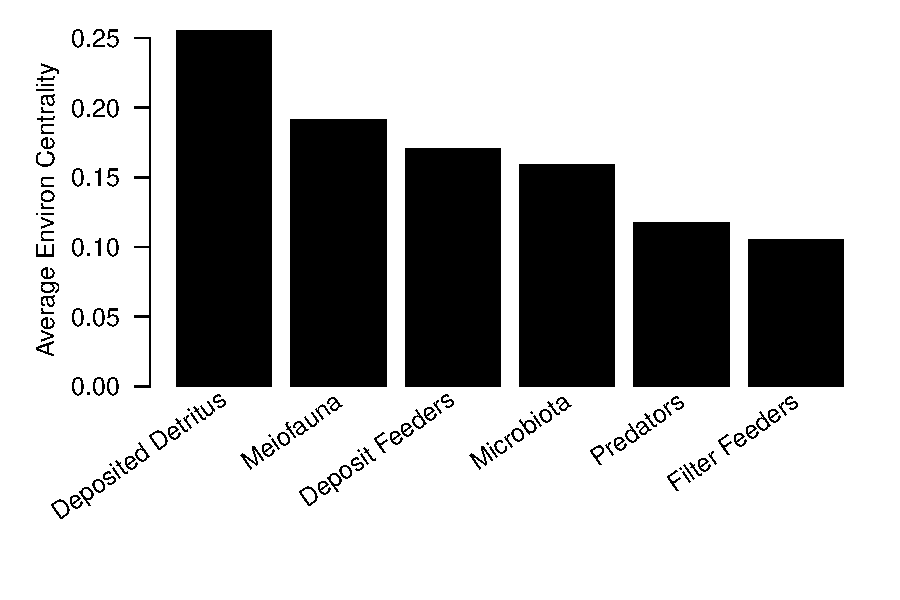
\includegraphics[]{enaR-vignette-039}
\caption{Bar plot of the Oyster Reef model Average Environ
  Centralities.} \label{fig:aec}
\end{figure}

\subsection{Output Orientation}  \label{sec:orient}

To facilitate package use by the existing ENA community, some of which
use the column-to-row orientation (e.g. the Patten School), we have
created orientation functions that enable the user to set the expected
output orientation for functions written in a particular ``school'' of
analysis. Thus, functions from either school will receive network
models with the standard row-to-column, but will return output with
flow matrices oriented in the column-to-row orientation when
appropriate (i.e. Patten school functions) and return them in that
same orientation.

Here is an example of how to use the model orientation functions to
re-orient the output from \texttt{enaFlow}:

\begin{Schunk}
\begin{Sinput}
> ###Check the current orientation
> get.orient()
> ###enaFlow output in row-column
> flow.rc <- enaFlow(oyster)$G
> ###Set the global orientation to school
> set.orient('school')
> ###Check that it worked
> get.orient()
> ###enaFlow output in column-row
> flow.cr <- enaFlow(oyster)$G
> ###Check. Outputs should be transposed from each other.
> all(flow.rc == flow.cr)
> all(flow.rc == t(flow.cr))
> ###Now change back to the default orientation ('rc')
> set.orient('rc')
> 
\end{Sinput}
\end{Schunk}


%% We close the description of the package's core functionality with a
%% plot of how the functions relate to each other and are supported by
%% helper functions (Fig.~\ref{fig:fig}).


\section{Model Library}

The \textit{enaR} package includes a library of 100 empirically based
ecosystem models. There are two general classes of ecosystem models.
First, there are 58 of the models are trophically-based models with
food webs at their core (Tables~\ref{tab:TRO}).  Second, there are 42
models are focused on biogeochemical cycling in ecosystems
(Table~\ref{tab:BGC}).  \citet{christian96}, \citet{baird08_sylt}, and
\citet{borrett10_idd} have previously suggested this model class
distinction.  In summary, these models were originally published for a
number of different types of ecosystems, though predominantly aquatic,
by a number of author teams.  Models in the library range in size from
4 nodes to 125 nodes with connectance values ranging from 7\% to 45\%.

This collection of models overlaps with other data sets.  For example,
twenty-seven of the models (47\%) are included in the set of models
compiled and distributed by Dr. Ulanowicz
(\href{http://www.cbl.umces.edu/~ulan/ntwk/network.html}{http://www.cbl.umces.edu/~ulan/ntwk/network.html}).
All 50 of the models analyzed by \citet{borrett10_hmg} and
\citet{salas11_did} and the 45 models analyzed in \citet{borrett13}
are included in this model library.

The trophic models are grouped as the \texttt{troModels} object and
the biogeochemically-based models are available as the
\texttt{bgcModels} object.  Both data objects return a list of the
model network objects.  To use these models simply use the R
\textit{base} \texttt{data} function. This will load the models into
the working memory as a named list of network objects:

\begin{Schunk}
\begin{Sinput}
> ### Import the model sets
> data(bgcModels)
> data(troModels)
> ### Check the first few model names
> head(names(bgcModels))
> head(names(troModels))
> ### Isolate a single model
> x <- troModels[[1]]
> x <- troModels$"Marine Coprophagy (oyster)"
> ### Check out the model
> summary(x)
\end{Sinput}
\end{Schunk}

%% ------- MODEL TABLES ------------ %%

% Thu May  2 13:54:17 2013
\begin{table}[ht]
\begin{center}
  \caption{Trophic ecosystem networks (58) included in the
    \textit{enaR} model library.} \label{tab:TRO}
  \begin{tiny}
    \begin{tabular}{llrrrrrr}
      \hline
      Models & Units & $n^\dagger$ & $C^\dagger$ & $Input^\dagger$ & $TST^\dagger$ & $FCI^\dagger$ & Reference \\
      \hline
      Marine Coprophagy (oyster) & kcal m$^{-2}$ yr$^{-1}$  &   4 & 0.25 & 379 & 549 & 0.12 & \citet{haven66} \\
      Lake Findley  & gC m$^{-2}$ yr$^{-1}$  &   4 & 0.38 &  21 &  50 & 0.30 &  \citet{richey78} \\
      Mirror Lake & gC m$^{-2}$ yr$^{-1}$  &   5 & 0.36 &  72 & 217 & 0.32 &   \citet{richey78} \\
      Lake Wingra & gC m$^{-2}$ yr$^{-1}$  &   5 & 0.40 & 478 & 1517 & 0.40 &  \citet{richey78} \\
      Marion Lake & gC m$^{-2}$ yr$^{-1}$  &   5 & 0.36 &  87 & 242 & 0.31 &  \citet{richey78} \\
      Cone Springs & kcal m$^{-2}$ yr$^{-1}$  &   5 & 0.32 & 11819 & 30626 & 0.09 &  \citet{tilly68} \\
      Silver Springs & kcal m$^{-2}$ yr$^{-1}$  &   5 & 0.28 & 21296 & 29175 & 0.00 &  \citet{odum57} \\
      English Channel & kcal m$^{-2}$ yr$^{-1}$  &   6 & 0.25 & 1096 & 2280 & 0.00 &  \citet{brylinsky72} \\
      Oyster Reef  & kcal m$^{-2}$ yr$^{-1}$  &   6 & 0.33 &  41 &  83 & 0.11 &  \citet{dame81} \\
      Baie de Somme & mgC m$^{-2}$ d$^{-1}$  &   9 & 0.30 & 876 & 2034 & 0.14 &  \citet{rybarczyk03} \\
      Bothnian Bay & gC m$^{-2}$ yr$^{-1}$  &  12 & 0.22 &  44 & 183 & 0.23 &   \citet{sandberg00} \\
      Bothnian Sea & gC m$^{-2}$ yr$^{-1}$  &  12 & 0.24 & 117 & 562 & 0.31 &   \citet{sandberg00} \\
      Ythan Estuary & gC m$^{-2}$ yr$^{-1}$  &  13 & 0.23 & 1258 & 4181 & 0.24 &  \citet{baird81} \\
      Sundarban Mangrove (virgin) & kcal m$^{-2}$ yr$^{-1}$  &  14 & 0.22 & 111317 & 440931 & 0.19 & \citet{ray08} \\
      Sundarban Mangrove (reclaimed) & kcal m$^{-2}$ yr$^{-1}$  &  14 & 0.22 & 38484 & 103056 & 0.05 & \citet{ray08} \\
      Baltic Sea & mg C m$^{-2}$ d$^{-1}$  &  15 & 0.17 & 603 & 1973 & 0.13 &   \citet{baird91} \\
      Ems Estuary & mg C m$^{-2}$ d$^{-1}$  &  15 & 0.19 & 282 & 1067 & 0.32 &  \citet{baird91} \\
      Swartkops Estuary  15 & mg C m$^{-2}$ d$^{-1}$  &  15 & 0.17 & 3544 & 13996 & 0.47 &   \citet{baird91} \\
      Southern Benguela Upwelling & mg C m$^{-2}$ d$^{-1}$  &  16 & 0.23 & 714 & 2545 & 0.31 & \citet{baird91} \\
      Peruvian Upwelling & mg C m$^{-2}$ d$^{-1}$  &  16 & 0.22 & 14927 & 33491 & 0.04 &  \citet{baird91} \\
      Crystal River (control) & mg C m$^{-2}$ d$^{-1}$  &  21 & 0.19 & 7357 & 15062 & 0.07 &  \citet{ulanowicz86} \\
      Crystal River (thermal) & mg C m$^{-2}$ d$^{-1}$  &  21 & 0.14 & 6018 & 12032 & 0.09 &  \citet{ulanowicz86} \\
      Charca de Maspalomas Lagoon & mg C m$^{-2}$ d$^{-1}$  &  21 & 0.12 & 1486230 & 6010331 & 0.18 &  \citet{almunia99} \\
      Northern Benguela Upwelling & mg C m$^{-2}$ d$^{-1}$  &  24 & 0.21 & 2282 & 6611 & 0.05 &  \citet{heymans00} \\
      Swartkops Estuary & mg C m$^{-2}$ d$^{-1}$  &  25 & 0.17 & 2859 & 8949 & 0.27 & \citet{scharler05} \\
      Sunday Estuary & mg C m$^{-2}$ d$^{-1}$  &  25 & 0.16 & 4440 & 11937 & 0.22 & \citet{scharler05} \\
      Kromme Estuary & mg C m$^{-2}$ d$^{-1}$  &  25 & 0.16 & 2571 & 11087 & 0.38 & \citet{scharler05} \\
      Okefenokee Swamp & g dw m$^{-2}$ y$^{-1}$  &  26 & 0.20 & 2533 & 12855 & 0.48 & \citet{whipple93} \\
      Neuse Estuary (early summer 1997) & mg C m$^{-2}$ d$^{-1}$  &  30 & 0.09 & 4385 & 13827 & 0.12 &  \citet{baird04} \\
      Neuse Estuary (late summer 1997)  & mg C m$^{-2}$ d$^{-1}$  &  30 & 0.11 & 4639 & 13035 & 0.13 &  \citet{baird04} \\
      Neuse Estuary (early summer 1998) & mg C m$^{-2}$ d$^{-1}$  &  30 & 0.09 & 4568 & 14025 & 0.12 &  \citet{baird04} \\
      Neuse Estuary (late summer 1998) & mg C m$^{-2}$ d$^{-1}$  &  30 & 0.10 & 5641 & 15031 & 0.11 &  \citet{baird04} \\
      Gulf of Maine & g ww m$^{-2}$ yr$^{-1}$  &  31 & 0.35 & 5053 & 18381 & 0.15 &   \citet{link08} \\
      Georges Bank & g ww m$^{-2}$ yr$^{-1}$  &  31 & 0.35 & 4380 & 16889 & 0.18 &  \citet{link08} \\
      Middle Atlantic Bight & g ww m$^{-2}$ yr$^{-1}$  &  32 & 0.37 & 4869 & 17916 & 0.18 &  \citet{link08} \\
      Narragansett Bay & mgC m$^{-2}$ yr$^{-1}$  &  32 & 0.15 & 693845 & 3917246 & 0.51 &  \citet{monaco97} \\
      Southern New England Bight & g ww m$^{-2}$ yr$^{-1}$  &  33 & 0.35 & 4717 & 17597 & 0.16 &  \citet{link08} \\
      Chesapeake Bay  & mg C m$^{-2}$ yr$^{-1}$  &  36 & 0.09 & 888791 & 3227453 & 0.19 &  \citet{baird89} \\
      Mondego Estuary (\textit{Zostera} sp. Meadows) & g AFDW m$^{−2}$ yr$^{−1}$ &  43 & 0.19 & 4030 & 6822 & 0.03 & \citet{patricio2006mass} \\
      St. Marks Seagrass, site 1 (Jan.) & mg C m$^{-2}$ d$^{-1}$  &  51 & 0.08 & 514 & 1315 & 0.13 &  \citet{baird98} \\
      St. Marks Seagrass, site 1 (Feb.) & mg C m$^{-2}$ d$^{-1}$  &  51 & 0.08 & 601 & 1590 & 0.11 &  \citet{baird98} \\
      St. Marks Seagrass, site 2 (Jan.) & mg C m$^{-2}$ d$^{-1}$  &  51 & 0.07 & 602 & 1383 & 0.09 &  \citet{baird98} \\
      St. Marks Seagrass, site 2 (Feb.) & mg C m$^{-2}$ d$^{-1}$  &  51 & 0.08 & 800 & 1921 & 0.08 &  \citet{baird98} \\
      St. Marks Seagrass, site 3 (Jan.) & mg C m$^{-2}$ d$^{-1}$  &  51 & 0.05 & 7809 & 12651 & 0.01 & \citet{baird98} \\
      St. Marks Seagrass, site 4 (Feb.) & mg C m$^{-2}$ d$^{-1}$  &  51 & 0.08 & 1432 & 2865 & 0.04 &  \citet{baird98} \\
      Sylt-R{\o}m{\o} Bight & mg C m$^{-2}$ d$^{-1}$  &  59 & 0.08 & 683448 & 1781028 & 0.09 &  \citet{baird04_sylt} \\
      Graminoids (wet) & g C m$^{-2}$ yr$^{-1}$  &  66 & 0.18 & 6272 & 13676 & 0.02 &  \citet{ulanowicz00_graminoids} \\
      Graminoids (dry) & g C m$^{-2}$ yr$^{-1}$  &  66 & 0.18 & 3472 & 7519 & 0.04 &   \citet{ulanowicz00_graminoids} \\
      Cypress (wet) & g C m$^{-2}$ yr$^{-1}$  &  68 & 0.12 & 1418 & 2571 & 0.04 &  \citet{ulanowicz97_cypress} \\
      Cypress (dry) & g C m$^{-2}$ yr$^{-1}$  &  68 & 0.12 & 1035 & 1919 & 0.04 &  \citet{ulanowicz97_cypress} \\
      Lake Oneida (pre-ZM) & g C m$^{-2}$ yr$^{-1}$  &  74 & 0.22 & 1034 & 1697 & 0.00 &  \citet{miehls09_oneida} \\
      Lake Oneida (post-ZM) & g C m$^{-2}$ yr$^{-1}$  &  76 & 0.22 & 810 & 1462 & 0.00 &  \citet{miehls09_oneida} \\
      Bay of Quinte (pre-ZM) & g C m$^{-2}$ yr$^{-1}$  &  74 & 0.21 & 984 & 1509 & 0.00 &   \citet{miehls09_quinte} \\
      Bay of Quinte (post-ZM) & g C m$^{-2}$ yr$^{-1}$  &  80 & 0.21 & 1129 & 2039 & 0.01 &   \citet{miehls09_quinte} \\
      Mangroves (wet) & g C m$^{-2}$ yr$^{-1}$  &  94 & 0.15 & 1531 & 3265 & 0.10 &  \citet{ulanowicz99_mangrove} \\
      Mangroves (dry) & g C m$^{-2}$ yr$^{-1}$  &  94 & 0.15 & 1531 & 3272 & 0.10 &  \citet{ulanowicz99_mangrove} \\
      Florida Bay (wet) & mg C m$^{-2}$ yr$^{-1}$  & 125 & 0.12 & 738 & 2720 & 0.14 &  \citet{ulanowicz98_fb} \\
      Florida Bay (dry) & mg C m$^{-2}$ yr$^{-1}$  & 125 & 0.13 & 547 & 1778 & 0.08 &  \citet{ulanowicz98_fb} \\
      \hline
\end{tabular}
\end{tiny}
\end{center}
\begin{scriptsize}
  $^\dagger$ $n$ is the number of nodes in the network model,
  $C=L/n^2$ is the model connectance when $L$ is the number of direct
  links or energy--matter transfers, $Input =sum{z_i}$ is the total
  amount of energy--matter flowing into the system,
  $TST=\sum\sum{f_{ij}}+\sum{z_i}$ is the total system throughflow,
  and $FCI$ is the Finn Cycling Index \citep{finn80}. Flow based
  network statistics ($Input$, $TST$, and $FCI$) were calculated after
  models were balanced using the AVG2 algorithm.
\end{scriptsize}
\end{table}

% -- BGC Table --- %
\begin{table}[ht]
\begin{center}
  \caption{Biogeochemical ecosystem networks (42) included in the
    \textit{enaR} model library.} \label{tab:BGC}
  \begin{tiny}
    \begin{tabular}{llrrrrrr}
      \hline
      Model & Units & $n^\dagger$ & $C^\dagger$ & $Input^\dagger$ & $TST^\dagger$ & $FCI^\dagger$ & Reference \\
      \hline
      Hubbard Brook (Waide) & kg Ca Ha$^{-1}$  yr$^{-1}$ &   4 & 0.25 &  11 & 168 & 0.76 & \citet{waide74} \\
      Hardwood Forest, NH & kg Ca Ha$^{-1}$  yr$^{-1}$ &   4 & 0.31 &  11 & 200 & 0.80 & \citet{jordan72} \\
      Douglas Fir Forest, WA  & kg Ca Ha$^{-1}$  yr$^{-1}$ &   4 & 0.31 &   4 &  54 & 0.74 & \citet{jordan72} \\
      Douglas Fir Forest, WA  & kg K Ha$^{-1}$  yr$^{-1}$ &   4 & 0.31 &   0 &  45 & 0.97 & \citet{jordan72} \\
      Puerto Rican Rain Forest & kg Ca Ha$^{-1}$  yr$^{-1}$ &   4 & 0.31 &  43 & 274 & 0.57 & \citet{jordan72} \\
      Puerto Rican Rain Forest & kg K Ha$^{-1}$  yr$^{-1}$ &   4 & 0.31 &  20 & 433 & 0.86 & \citet{jordan72} \\
      Puerto Rican Rain Forest & kg Mg Ha$^{-1}$  yr$^{-1}$ &   4 & 0.31 &  10 &  70 & 0.58 & \citet{jordan72} \\
      Puerto Rican Rain Forest & kg Cu Ha$^{-1}$  yr$^{-1}$ &   4 & 0.31 &   0 &   2 & 0.37 & \citet{jordan72} \\
      Puerto Rican Rain Forest & kg Fe Ha$^{-1}$  yr$^{-1}$ &   4 & 0.31 &   0 &   7 & 0.95 & \citet{jordan72} \\
      Puerto Rican Rain Forest & kg Mn Ha$^{-1}$  yr$^{-1}$ &   4 & 0.38 &   0 &   7 & 0.98 & \citet{jordan72} \\
      Puerto Rican Rain Forest & kg Na Ha$^{-1}$  yr$^{-1}$ &   4 & 0.31 &  64 & 140 & 0.24 & \citet{jordan72} \\
      Puerto Rican Rain Forest & kg Sr Ha$^{-1}$  yr$^{-1}$ &   4 & 0.31 &   0 &   1 & 0.71 & \citet{jordan72} \\
      Tropical Rain Forest & g N m$^{-2}$ d$^{-1}$  &   5 & 0.24 &  10 &  71 & 0.48 & \citet{edmisten70} \\
      Neuse River Estuary (AVG) & mmol N m$^{-2}$ season$^{-1}$ &   7 & 0.45 & 795 & 41517 & 0.89 & \citet{christian03} \\
      Neuse River Estuary (Spring 1985) & mmol N m$^{-2}$ season$^{-1}$ &   7 & 0.45 & 133 & 9120 & 0.91 & \citet{christian03} \\
      Neuse River Estuary (Summer 1985) & mmol N m$^{-2}$ season$^{-1}$ &   7 & 0.45 & 119 & 20182 & 0.96 & \citet{christian03} \\
      Neuse River Estuary Fall 1985) & mmol N m$^{-2}$ season$^{-1}$ &   7 & 0.45 & 181 & 8780 & 0.88 & \citet{christian03} \\
      Neuse River Estuary Winter 1986) & mmol N m$^{-2}$ season$^{-1}$ &   7 & 0.43 & 187 & 6880 & 0.85 & \citet{christian03} \\
      Neuse River Estuary (Spring 1986) & mmol N m$^{-2}$ season$^{-1}$ &   7 & 0.45 & 128 & 12915 & 0.94 & \citet{christian03} \\
      Neuse River Estuary (Summer 1986) & mmol N m$^{-2}$ season$^{-1}$ &   7 & 0.45 & 165 & 11980 & 0.91 & \citet{christian03} \\
      Neuse River Estuary (Fall 1986) & mmol N m$^{-2}$ season$^{-1}$ &   7 & 0.45 & 100 & 9863 & 0.94 & \citet{christian03} \\
      Neuse River Estuary (Winter 1987) & mmol N m$^{-2}$ season$^{-1}$ &   7 & 0.45 & 691 & 7907 & 0.62 & \citet{christian03} \\
      Neuse River Estuary (Spring 1987) & mmol N m$^{-2}$ season$^{-1}$ &   7 & 0.45 & 334 & 11533 & 0.84 & \citet{christian03} \\
      Neuse River Estuary (Summer 1987) & mmol N m$^{-2}$ season$^{-1}$ &   7 & 0.45 &  90 & 15621 & 0.96 & \citet{christian03} \\
      Neuse River Estuary (Fall 1987) & mmol N m$^{-2}$ season$^{-1}$ &   7 & 0.45 &  85 & 7325 & 0.93 & \citet{christian03} \\
      Neuse River Estuary (Winter 1988) & mmol N m$^{-2}$ season$^{-1}$ &   7 & 0.45 & 171 & 8680 & 0.89 & \citet{christian03} \\
      Neuse River Estuary (Spring 1988) & mmol N m$^{-2}$ season$^{-1}$ &   7 & 0.45 & 176 & 6898 & 0.85 & \citet{christian03} \\
      Neuse River Estuary (Summer 1988) & mmol N m$^{-2}$ season$^{-1}$ &   7 & 0.45 & 132 & 16814 & 0.95 & \citet{christian03} \\
      Neuse River Estuary (Fall 1988) & mmol N m$^{-2}$ season$^{-1}$ &   7 & 0.45 & 128 & 5732 & 0.87 & \citet{christian03} \\
      Neuse River Estuary (Winter 1989) & mmol N m$^{-2}$ season$^{-1}$ &   7 & 0.45 & 291 & 5739 & 0.75 & \citet{christian03} \\
      Cape Fear River Estuary (Oligohaline) & nmol N cm$^{-3}$ d$^{-1}$ &   8 & 0.36 & 3802 & 7088 & 0.20 & \citet{hines12} \\
      Cape Fear River Estuary (Polyhaline) & nmol N cm$^{-3}$ d$^{-1}$ &   8 & 0.36 & 3068 & 5322 & 0.17 & \citet{hines2015} \\
      Lake Lanier (AVG) & mg P m$^{-2}$ day$^{-1}$ &  11 & 0.21 &  95 & 749 & 0.40 & \citet{borrett07_lanier} \\
      Baltic Sea & mg N m$^{-3}$ day$^{-1}$  &  16 & 0.15 & 2348 & 44510 & 0.67 & \citet{hinrichsen98_baltic} \\
      Chesapeake Bay & mg N m$^{-2}$ yr$^{-1}$  &  36 & 0.12 & 73430 & 484325 & 0.33 & \citet{baird95} \\
      Chesapeake Bay & mg P m$^{-2}$ yr$^{-1}$ &  36 & 0.12 & 9402 & 101091 & 0.51 & \citet{ulanowicz99} \\
      Chesapeake Bay (Winter) & mg P m$^{-2}$ season$^{-1}$ &  36 & 0.08 & 1009 & 11926 & 0.53 & \citet{ulanowicz99} \\
      Chesapeake Bay (Spring) & mg P m$^{-2}$ season$^{-1}$ &  36 & 0.10 & 1932 & 27325 & 0.57 & \citet{ulanowicz99} \\
      Chesapeake Bay (Summer) & mg P m$^{-2}$ season$^{-1}$ &  36 & 0.12 & 4184 & 42935 & 0.46 & \citet{ulanowicz99} \\
      Chesapeake Bay (Fall) & mg P m$^{-2}$ season$^{-1}$ &  36 & 0.10 & 2276 & 18904 & 0.40 & \citet{ulanowicz99} \\
      Sylt-R{\o}m{\o} Bight & mg N m$^{-2}$ yr$^{-1}$  &  59 & 0.09 & 99613 & 363693 & 0.23 & \citet{baird08_sylt} \\
      Sylt-R{\o}m{\o} Bight & mg P m$^{-2}$ yr$^{-1}$  &  59 & 0.09 & 2508 & 57739 & 0.66 & \citet{baird08_sylt} \\
      \hline
    \end{tabular}
  \end{tiny}
\end{center}
\begin{scriptsize}
  $^\dagger$ $n$ is the number of nodes in the network model,
  $C=L/n^2$ is the model connectance when $L$ is the number of direct
  links or energy--matter transfers, $Input =sum{z_i}$ is the total
  amount of energy--matter flowing into the system,
  $TST=\sum\sum{f_{ij}}+\sum{z_i}$ is the total system throughflow,
  and $FCI$ is the Finn Cycling Index \citep{finn80}. Flow based
  network statistics ($Input$, $TST$, and $FCI$) were calculated after
  models were balanced using the AVG2 algorithm.
\end{scriptsize}
\end{table}


%%%%%%%%%%%%%%%%%%%%%%%%%%%%%%%%%%%%%%%%%%%%%%%%%%%%%%%%%
\section{Multi-Model Analyses (Batch Processing)}

While many investigators analyze single models, much of ENA is used to
compare ecosystem models \citep[e.g.,][]{baird91, baird95, christian03,
  whipple07}.  Investigators have also analyzed large set of models to
determine the generality of hypothesized ecosystem properties
\citep[e.g.,][]{christensen95, borrett10_hmg, salas11_did}.  For both
of these applications, investigators need to analyze multiple models.
One advantage of the \textit{enaR} \R\ package is that it simplifies this
batch processing.  Here we illustrate how to batch analyze a
selection of models.

Our first step is to read in the model data for a set of trophic
models:

\begin{Schunk}
\begin{Sinput}
> data(troModels)
\end{Sinput}
\end{Schunk}


Now that we have the raw data loaded, we can start to manipulate
it.  The first step is to balance the models and then we can run the
flow analysis.  We are using the \texttt{lapply} function to apply the
analysis across the list of models stored in model.list.

%%%Working on pairing down the balancing example run time

\begin{Schunk}
\begin{Sinput}
> # balance models as necessary
> m.list <- lapply(troModels[1:10],balance)
> # check that models are balanced
> unlist(lapply(m.list,ssCheck))
> # if balancing fails, you can use force.balance
> # to repeatedly apply the balancing procedure
> # although this is not the case with our model set
> 
> m.list <- lapply(m.list,force.balance)
> ##Check that all the models are balanced
> all(unlist(lapply(m.list,ssCheck)))
> # Example Flow Analysis
> F.list <- lapply(m.list, enaFlow)
> # the full results of the flow analysis is now stored in the elements
> # of the F.list.  To get the results for just the first model...
> F.list[[1]]
> 
\end{Sinput}
\end{Schunk}

We can use the same technique to extract specific information, like
just the ratio of Indirect-to-Direct flow for each model.


\begin{Schunk}
\begin{Sinput}
> # Example of extracting just specific information - Indirect Effects Ratio
> IDs <- unlist(lapply(m.list, function(x) enaFlow(x)$ns[8]))
> #Look at the first few ID's
> head(IDs)
\end{Sinput}
\end{Schunk}

We can also collect the set of output-oriented integral flow matrices.
\begin{Schunk}
\begin{Sinput}
> # Here is a list containing only the output-oriented integral flow matrices
> N.list <- lapply(m.list,function(x) enaFlow(x)$N)
\end{Sinput}
\end{Schunk}

We can also apply the \texttt{get.ns} function to extract all of the
network statistics for each model.  We then use the \texttt{do.call}
function to reshape the network statistics into a single data frame.

\begin{Schunk}
\begin{Sinput}
> # Collecting and combining all network statistics
> ns.list <- lapply(m.list,get.ns) # returns as list
> ns <- do.call(rbind,ns.list)  # ns as a data.frame
> # Let's take a quick look at some of the output
> colnames(ns)    # return network statistic names.
> dim(ns)         # show dimensions of ns matrix
> ns[1:5,1:5]     # show selected results
\end{Sinput}
\end{Schunk}

Given this data frame of network statistics, we can construct
interesting plots for further analysis. Here we focus on results of
the St.\ Marks Seagrass ecosystem \citep{baird98}.


\begin{Schunk}
\begin{Sinput}
> opar <- par(las=1,mar=c(9,7,2,1),xpd=TRUE,mfrow=c(1,2),oma=c(1,1,0,0))
> x=dim(ns)[1] # number of models
> m.select <- 40:45
> bp=barplot(ns$ID.F[m.select],ylab="Indirect-to-Direct Flow Ratio (I/D, Realized)",
+         col="darkgreen",border=NA,ylim=c(0,2))
> text(bp,-0.05,                # add labels
+      labels=rownames(ns)[m.select],
+        srt=45,adj=1,cex=0.85)
> opar <- par(xpd=FALSE)
> abline(h=1,col="orange",lwd=2)
> #
> plot(ns$FCI,ns$ID.F,pch=20,col="blue",cex=2,
+      ylab="Indirect-to-Direct Flow Ratio (I/D, Realized)",
+      xlab="Finn Cycling Index (FCI)",
+      xlim=c(0,0.8),ylim=c(0,8))
> #
> rm(opar)  # remove the plotting parameters
\end{Sinput}
\end{Schunk}


\begin{figure}
  \center
%% <<fig=true,echo=false>>=
%% <<b>>
%% @
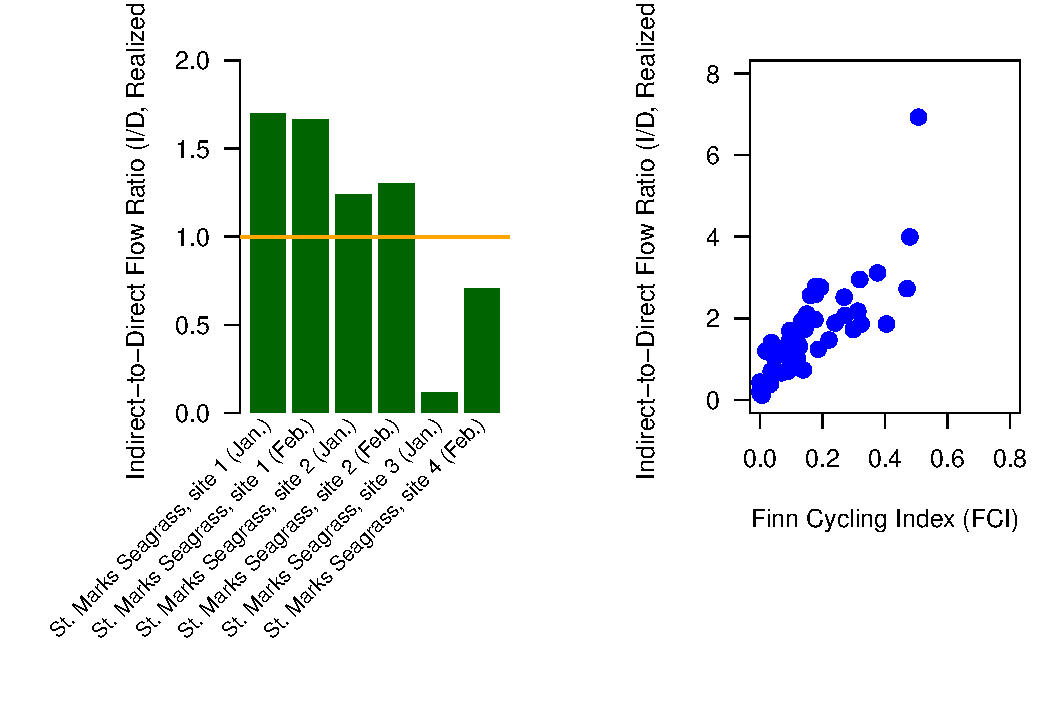
\includegraphics[]{enaR-vignette-048}
\caption{Ratio of Indirect-to-Direct Flow for six ecosystem models
  (left) and relationship between the Finn Cycling Index and the ratio
  of Indirect-to-Direct flow in the 56 trophic models.} \label{fig:aec}
\end{figure}


\section{Connecting to Other Useful Packages}
Another advantage of building the \textit{enaR} package in \R\ is that
it lets ecologists take advantage of other types of network analysis
and statistical tools that already exist in \R.  We highlight two
examples here.

\subsection{sna: Social Network Analysis}
The \textit{sna} package for Social Network Analysis is bundled in the
\textit{statnet} package and uses the same network data object defined
in \textit{network} that we selected to use for \textit{enaR}.  Thus,
the design decision to use the network data object gives users direct
access to \textit{sna} tools.

Multiple measures of network centrality have been proposed, and the
\textit{sna} package provides a way of calculating several.  Thus,
ecologists can now use the sna algorithms to determine different types
of centrality for their models.

\begin{Schunk}
\begin{Sinput}
> betweenness(oyster)
> closeness(oyster)
\end{Sinput}
\end{Schunk}

The \textit{sna} package introduced new graphical capabilities as
well. For example, it will create a target diagram of centralities.
%%\afterpage{\clearpage}

%%%FIX ME!!!

\begin{Schunk}
\begin{Sinput}
> m <- troModels[[38]]
> b <- betweenness(m)         # calculate betweenness centrality
> nms <- m%v%'vertex.names'   # get vertex names
> show(nms)
> nms[b<=(0.1*max(b))] <- NA  # exclude less central nodes
> set.seed(3)
> opar <- par(xpd=TRUE,mfrow=c(1,1))
> # create target plot
> gplot.target(m,b,#circ.lab=FALSE,
+              edge.col="grey",
+              label=nms) # show only labels of most central nodes
>              #xlim=c(-1,4))
> rm(opar)
\end{Sinput}
\end{Schunk}

\begin{figure}[!htbp]
  \center
%% <<fig=true,echo=false,eval=true>>=
%% <<d>>
%% @
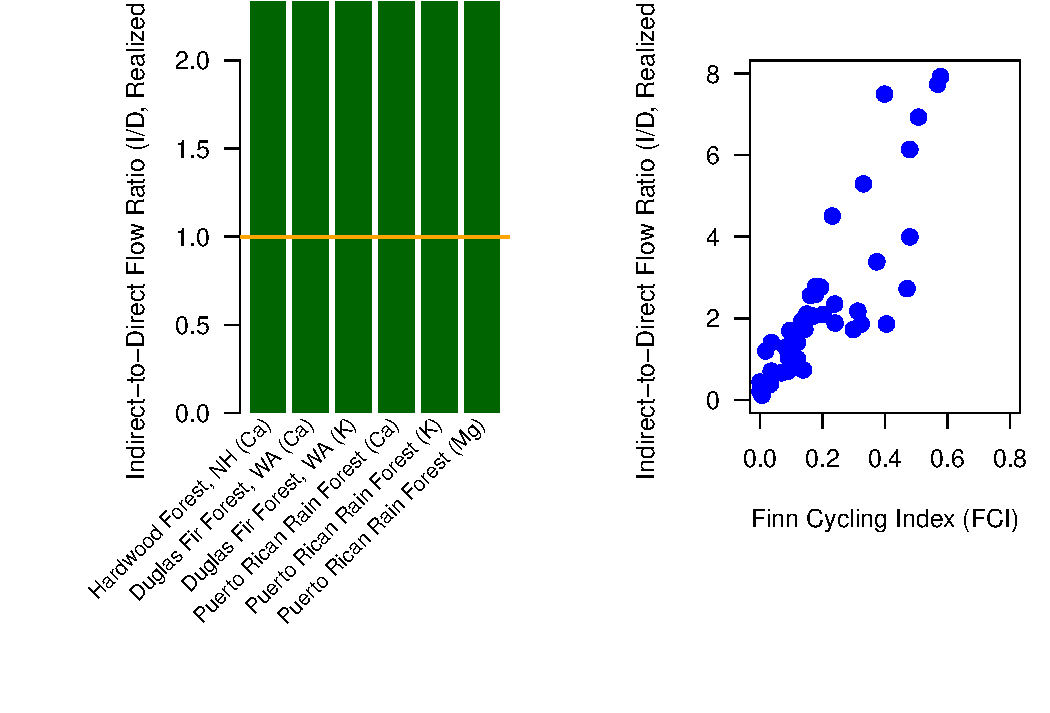
\includegraphics[]{enaR-vignette-051}
\caption{Target plot of node betweenness centrality for the Chesapeake
  Bay model (mesohaline, carbon, annual).} \label{fig:target}
\end{figure}


In addition to the node-level measures, \textit{sna} includes graph-level
indices.

\begin{Schunk}
\begin{Sinput}
> centralization(oyster, degree)
> centralization(oyster,closeness)
> centralization(oyster,betweenness)
\end{Sinput}
\end{Schunk}

%%\afterpage{\clearpage}
%%%%%%%%%%%%%%%%%%%%%%%%%%%%%%%
\subsection{iGraph}
The \textit{iGraph} package can also be useful for analyzing network
data.  Here are a few examples of using the package.  Note that some
functions in \textit{iGraph} conflict with other functions already defined, so
care is required when using \textit{iGraph}.

%<<e,eval=true>>=
\begin{Schunk}
\begin{Sinput}
> library(igraph)
> ### The adjacency matrix
> A <- St$A
> ### creating an iGraph graph
> g <- graph.adjacency(A)
> plot(g)  # uses iGraph plot tools
\end{Sinput}
\end{Schunk}

\textit{iGraph} has a different set of visualization tools and
generates a different looking graph (Fig.~\ref{fig:igraph}).

\begin{figure}
\center
%% <<fig=TRUE,echo=false>>=
%% <<e>>
%% @
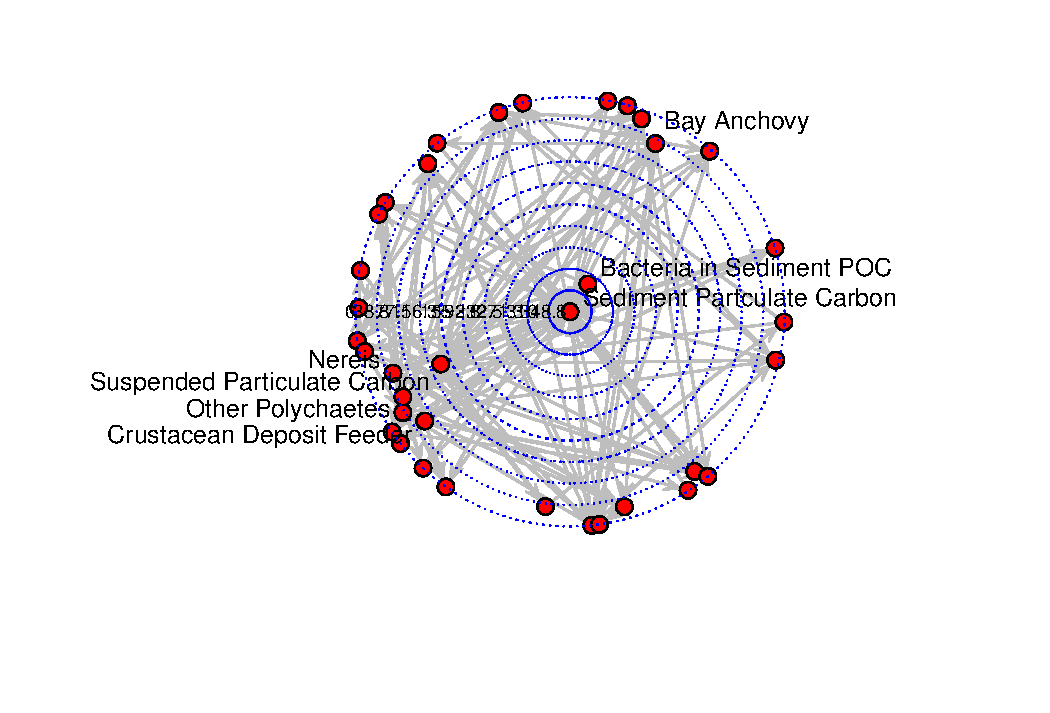
\includegraphics[]{enaR-vignette-054}
\caption{Plot of Oyster reef model using \textit{iGraph}}\label{fig:igraph}
\end{figure}

\begin{Schunk}
\begin{Sinput}
> # betweenness centrality (calculated by iGraph and sna)
> betweenness(g)
> # shortest path between any two nodes
> shortest.paths(g)
> # average path length in the network (graph theory sense)
> average.path.length(g,directed=TRUE)
> diameter(g)  # diameter of the graph
> vertex.connectivity(g)  # connectivity of a graph (group cohesion)
> subcomponent(g,1,'in')  # subcomponent reachable from 1 along inputs
> subcomponent(g,2,'in')  # subcomponent reachable from 2 along inputs
> subcomponent(g,1,'out') # subcomponent reachable from 1 along outputs
> subcomponent(g,2,'out') # subcomponent reachable from 2 along output
> edge.connectivity(g)
> detach(package:igraph)  # detach igraph package
\end{Sinput}
\end{Schunk}



There are other \R\ packages that have graph and network analysis tools,
like Bioconductor, that might also be useful for ecologists


\section{Summary and Future}
This vignette shows how to use several of the key features of the
\textit{enaR} package that enables scientists to perform Ecological
Network Analysis in \R.  The vision for this package is that it will
provide access to ENA algorithms from both the Ulanowicz and Patten
Schools.  In its current form it replicates, updates, and extends the
functionality of the NEA.m function \citep{fath06}.  It also includes
both ascendency calculations and mixed trophic impacts from the
Ulanowicz school of ENA, but there remains many possibilities for
future development.  We hope to do this in collaboration with
users. This vignette also illustrates how users can further analyze
their data with other \R\ packages for graph and network analysis like
\textit{sna} and \textit{iGraph}.  In summary, we hope you find this
package useful for your ENA needs.




\end{document}
